\documentclass[11pt,a4paper]{article}
\usepackage[utf8]{inputenc}
\usepackage[margin=1in]{geometry}
\usepackage{amsmath,amssymb}
\usepackage{booktabs}
\usepackage{tabularx}
\usepackage{longtable}
\usepackage{graphicx}
\usepackage{color}
\usepackage{xcolor}
\usepackage{hyperref}
\usepackage{listings}
\usepackage{tikz}
\usetikzlibrary{shapes.geometric, arrows, positioning, fit, backgrounds, calc}
\usepackage{float}
\usepackage{caption}

\hypersetup{
    colorlinks=true,
    linkcolor=blue,
    filecolor=magenta,      
    urlcolor=cyan,
    pdftitle={VisionDocPhi-3.5: Version 2 OCR-Adaptive Methodology Report},
    pdfpagemode=FullScreen,
}

% Colors
\definecolor{codegray}{rgb}{0.95,0.95,0.95}
\definecolor{codeborder}{rgb}{0.8,0.8,0.8}
\definecolor{commentgreen}{rgb}{0.133,0.545,0.133}
\definecolor{keywordblue}{rgb}{0.0,0.0,1.0}

% Code listing styles
\lstdefinestyle{mystyle}{
    backgroundcolor=\color{codegray},   
    commentstyle=\color{commentgreen},
    keywordstyle=\color{keywordblue},
    numberstyle=\tiny\color{gray},
    stringstyle=\color{purple},
    basicstyle=\ttfamily\small,
    breakatwhitespace=false,         
    breaklines=true,                 
    captionpos=b,                    
    keepspaces=true,                 
    numbers=none,                    
    numbersep=5pt,                  
    showspaces=false,                
    showstringspaces=false,
    showtabs=false,                  
    tabsize=2,
    frame=single,
    rulecolor=\color{codeborder}
}
\lstset{style=mystyle}

\begin{document}

\title{\textbf{VisionDocPhi-3.5: Version 2 OCR-Adaptive Methodology Report}}
\author{}
\date{}
\maketitle

\begin{abstract}
\textbf{Document purpose:} This report documents the theoretical design and implementation of the Version 2 (V2) agentic OCR-infusion pipeline for Document Visual Question Answering (DocVQA). It is intended for examiner review: to verify that the design rationale is sound, that the implementation matches the design, and that reported accuracy gains are real and measurable.

\vspace{0.2cm}
\noindent \textbf{Scope:} V2 pipeline only (evaluation output: \texttt{data/outputs/ocr\_adaptive\_200\_v2/}). Baseline comparison uses \texttt{data/outputs/baseline\_200/}. Code references point to the repository at commit \texttt{36e86b0} (``Ocr\_spatial\_improvement'').

\vspace{0.2cm}
\noindent \textbf{Base model:} \texttt{microsoft/phi-3.5-vision-instruct} (Phi-3.5-Vision) \\
\textbf{Dataset:} SP-DocVQA validation subset (200 stratified samples) \\
\textbf{OCR source:} Pre-extracted Azure Computer Vision JSON (\texttt{data/raw/spdocvqa\_ocr/})
\end{abstract}

\hrule
\vspace{0.5cm}

\section{Executive Summary}

\subsection{Problem}
Phi-3.5-Vision, used in zero-shot DocVQA mode, receives only a document image and a natural-language question. On dense structured documents (forms, tables, invoices), the model often:
\begin{itemize}
    \item Misreads fine print or handwritten digits.
    \item Selects the wrong field when many similar labels exist on the page.
    \item Hallucinates boilerplate text from headers or instruction regions.
\end{itemize}

\subsection{Proposed Solution}
An \textbf{agentic OCR-infusion pipeline} runs before VLM inference. Five specialized agents plus a quality gate decide \textbf{whether} to inject OCR text, \textbf{which lines} to inject, and \textbf{how} to format them. The VLM always receives the image; OCR is added as optional hints inside an XML wrapper when confidence is sufficient.

\subsection{Key Results (V2 vs. Baseline)}
Results from \texttt{data/outputs/comparisons/baseline\_vs\_adaptive\_report.json} are shown in Table~\ref{tab:key_results}.

\begin{table}[H]
\centering
\caption{Key Results (V2 vs. Baseline)}
\label{tab:key_results}
\begin{tabular}{|l|c|c|c|}
\hline
\textbf{Metric} & \textbf{Baseline (\texttt{vision\_only})} & \textbf{V2 OCR-Adaptive} & \textbf{Delta} \\ \hline
Mean ANLS & 0.506 & 0.658 & \textbf{+0.152} \\ \hline
Exact match rate & 0.420 & 0.595 & +0.175 \\ \hline
Layout-heavy cohort ANLS & 0.568 & 0.770 & +0.202 \\ \hline
Visual-heavy cohort ANLS & 0.444 & 0.546 & +0.102 \\ \hline
Per-sample wins & 6 (baseline) & 46 (adaptive) & 148 ties \\ \hline
\end{tabular}
\end{table}

\subsection{Critical Design Clarification}
\textbf{The Vision-Language Model (VLM) always generates the final answer.} There is no code path that returns OCR text directly without calling Phi-3.5-Vision. OCR infusion is \textbf{assistive multimodal fusion}: retrieved text with bounding-box coordinates is appended to the prompt alongside \texttt{<|image\_1|>}. When the quality gate rejects a snippet, inference falls back to image-only --- the same modality as baseline.

\newpage
\section{System Architecture}

\subsection{Baseline vs. V2 Adaptive --- High-Level Comparison}
Figure~\ref{fig:baseline_vs_adaptive} illustrates the contrast between the baseline mode and the V2 OCR-adaptive mode.

\begin{figure}[H]
\centering
\begin{tikzpicture}[node distance=1.5cm and 1.2cm, >=stealth, thick]
    % Styles for this diagram
    \tikzset{
        block/.style={rectangle, draw=blue!70!black, fill=blue!5, rounded corners, minimum height=2em, minimum width=8em, align=center, font=\small},
        decision/.style={diamond, draw=orange!70!black, fill=orange!5, aspect=2, minimum width=8em, align=center, font=\small},
        io/.style={trapezium, trapezium left angle=70, trapezium right angle=110, draw=green!60!black, fill=green!5, minimum height=2em, align=center, font=\small},
        line/.style={draw, ->, shorten >=1pt}
    }
    
    % --- BASELINE ---
    \node (BImg) [block] {Document Image};
    \node (BQ) [block, below=0.6cm of BImg] {Question};
    \node (BVLM) [block, right=1.5cm of ($(BImg.east)!0.5!(BQ.east)$)] {Phi-3.5-Vision};
    \node (BAns) [io, right=1cm of BVLM] {Answer};
    
    \path [line] (BImg.east) -- (BVLM.west);
    \path [line] (BQ.east) -- (BVLM.west);
    \path [line] (BVLM) -- (BAns);
    
    \pgfdeclarelayer{background}
    \pgfsetlayers{background,main}
    \begin{pgfonlayer}{background}
        \node[draw=gray, dashed, fill=gray!2, fit=(BImg) (BQ) (BVLM) (BAns), inner sep=0.3cm, rounded corners, label={[shift={(0, -0.1)}]above:Baseline Mode}] (BBox) {};
    \end{pgfonlayer}
    
    % --- ADAPTIVE ---
    \node (AImg) [block, below=2.5cm of BQ] {Document Image};
    \node (AQ) [block, below=0.6cm of AImg] {Question};
    \node (OCRJson) [block, below=0.6cm of AQ] {Azure OCR JSON};
    
    \node (Router) [block, right=1.2cm of ($(AImg.east)!0.5!(AQ.east)$)] {Router};
    \node (Retriever) [block, right=1.2cm of OCRJson] {Retriever};
    \node (Expander) [block, right=1cm of Retriever] {Expander};
    \node (Formatter) [block, right=1cm of Expander] {Formatter};
    \node (Gate) [decision, right=1cm of Formatter] {Quality Gate};
    
    \node (Snippet) [block, above right=0.4cm and 0.8cm of Gate] {OCR Snippet};
    \node (NoOCR) [block, below right=0.4cm and 0.8cm of Gate] {No Snippet};
    
    \node (AVLM) [block, right=1.2cm of ($(Snippet.east)!0.5!(NoOCR.east)$)] {Phi-3.5-Vision};
    \node (AAns) [io, right=1cm of AVLM] {Answer};
    
    \path [line] (AImg.east) -- (Router.west);
    \path [line] (AQ.east) -- (Router.west);
    \path [line] (OCRJson.east) -- (Retriever.west);
    \path [line] (Router.south) -- node [midway, right, font=\scriptsize] {ocr\_infused} (Retriever.north);
    \path [line] (Retriever) -- (Expander);
    \path [line] (Expander) -- (Formatter);
    \path [line] (Formatter) -- (Gate);
    \path [line] (Gate.north) |- node [near start, above, font=\scriptsize] {pass} (Snippet.west);
    \path [line] (Gate.south) |- node [near start, below, font=\scriptsize] {fail} (NoOCR.west);
    
    \path [line] (AImg.east) -- ++(0.4,0) |- (AVLM.west);
    \path [line] (AQ.east) -- ++(0.2,0) |- (AVLM.west);
    \path [line] (Snippet.east) -- (AVLM.west);
    \path [line] (NoOCR.east) -- (AVLM.west);
    \path [line] (AVLM) -- (AAns);
    
    \begin{pgfonlayer}{background}
        \node[draw=gray, dashed, fill=gray!2, fit=(AImg) (AQ) (OCRJson) (Router) (Retriever) (Expander) (Formatter) (Gate) (Snippet) (NoOCR) (AVLM) (AAns), inner sep=0.3cm, rounded corners, label={[shift={(0, -0.1)}]above:V2 OCR-Adaptive Mode}] (ABox) {};
    \end{pgfonlayer}
\end{tikzpicture}
\caption{Baseline vs. V2 Adaptive Mode Comparison}
\label{fig:baseline_vs_adaptive}
\end{figure}

\newpage
\subsection{V2 Agent Pipeline --- Internal Flow}
The pipeline is orchestrated by the \texttt{AgenticDocVQAPipeline} class inside \texttt{src/agents/pipeline.py}. The internal flow is diagrammed in Figure~\ref{fig:internal_flow}.

\begin{figure}[H]
\centering
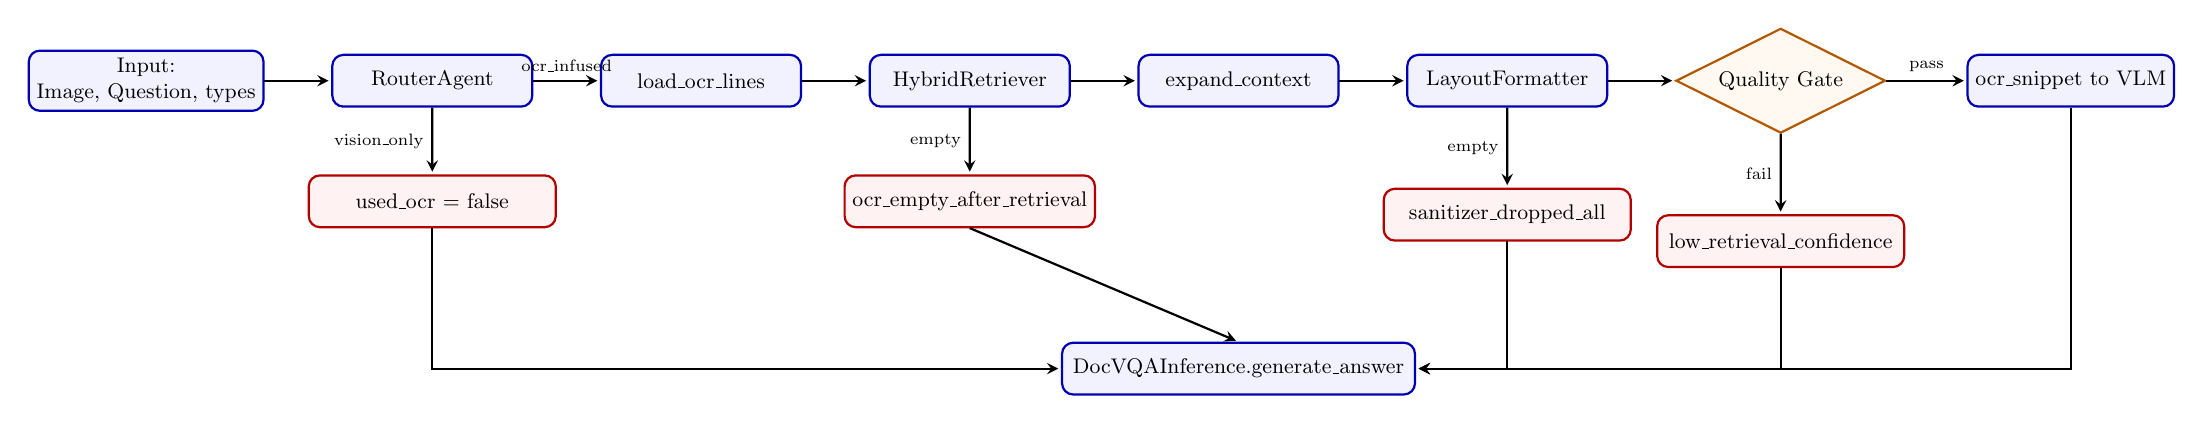
\begin{tikzpicture}[node distance=1.5cm and 0.6cm, >=stealth, thick, scale=0.85, every node/.style={transform shape}]
    \tikzset{
        block/.style={rectangle, draw=blue!70!black, fill=blue!5, rounded corners, minimum height=2.2em, minimum width=8.5em, align=center, font=\small},
        decision/.style={diamond, draw=orange!70!black, fill=orange!5, aspect=2, minimum width=8.5em, align=center, font=\small},
        exit/.style={rectangle, draw=red!70!black, fill=red!5, rounded corners, minimum height=2.2em, minimum width=10.5em, align=center, font=\small},
        line/.style={draw, ->, shorten >=1pt}
    }
    
    \node (Input) [block] {Input:\\Image, Question, types};
    \node (Router) [block, right=1.0cm of Input] {RouterAgent};
    \node (LoadOCR) [block, right=1.0cm of Router] {load\_ocr\_lines};
    \node (Retriever) [block, right=1.0cm of LoadOCR] {HybridRetriever};
    
    \node (Exit1) [exit, below=1cm of Router] {used\_ocr = false};
    \node (Exit2) [exit, below=1cm of Retriever] {ocr\_empty\_after\_retrieval};
    
    \node (Expander) [block, right=1.0cm of Retriever] {expand\_context};
    \node (Formatter) [block, right=1.0cm of Expander] {LayoutFormatter};
    \node (Gate) [decision, right=1.0cm of Formatter] {Quality Gate};
    
    \node (Exit3) [exit, below=1.2cm of Formatter] {sanitizer\_dropped\_all};
    \node (Exit4) [exit, below=1.2cm of Gate] {low\_retrieval\_confidence};
    \node (Success) [block, right=1.2cm of Gate] {ocr\_snippet to VLM};
    
    \node (VLM) [block, below=3.5cm of Expander, minimum width=15em] {DocVQAInference.generate\_answer};
    
    \path [line] (Input) -- (Router);
    \path [line] (Router) -- node [above, font=\scriptsize] {ocr\_infused} (LoadOCR);
    \path [line] (Router) -- node [left, font=\scriptsize] {vision\_only} (Exit1);
    \path [line] (LoadOCR) -- (Retriever);
    \path [line] (Retriever) -- node [left, font=\scriptsize] {empty} (Exit2);
    \path [line] (Retriever) -- (Expander);
    \path [line] (Expander) -- (Formatter);
    \path [line] (Formatter) -- (Gate);
    \path [line] (Formatter) -- node [left, font=\scriptsize] {empty} (Exit3);
    \path [line] (Gate) -- node [left, font=\scriptsize] {fail} (Exit4);
    \path [line] (Gate) -- node [above, font=\scriptsize] {pass} (Success);
    
    % Paths to VLM
    \path [line] (Exit1.south) |- (VLM.west);
    \path [line] (Exit2.south) -- (VLM.north);
    \path [line] (Exit3.south) |- (VLM.east);
    \path [line] (Exit4.south) |- (VLM.east);
    \path [line] (Success.south) |- (VLM.east);
    
\end{tikzpicture}
\caption{V2 Agent Pipeline: Internal Flow}
\label{fig:internal_flow}
\end{figure}

\subsection{Data Inputs}
The structure of inputs parsed by the pipeline is described in Table~\ref{tab:data_inputs}.

\begin{table}[H]
\centering
\caption{Data Inputs}
\label{tab:data_inputs}
\begin{tabular}{|p{3cm}|p{6cm}|p{6cm}|}
\hline
\textbf{Input} & \textbf{Source} & \textbf{Structure} \\ \hline
Document image & SP-DocVQA images (\texttt{data/raw/spdocvqa\_images/}) & PIL Image \\ \hline
Question & Dataset annotation & String \\ \hline
Question types & DocVQA metadata (eval only) & e.g., \texttt{["form"]}, \texttt{["figure/diagram"]} \\ \hline
OCR lines & Azure JSON via \texttt{src/data/ocr\_loader.py} & \texttt{OcrLine(line\_id, text, bbox=[x1,y1,x2,y2])} \\ \hline
\end{tabular}
\end{table}

The Azure \texttt{boundingBox} (8-point polygon) is converted to an axis-aligned \texttt{[x1, y1, x2, y2]} box by the function \texttt{bounding\_box\_to\_xyxy()}.

\subsection{Implementation Entry Point}
During evaluation, the method \texttt{DocVQAInference.evaluate()} in \texttt{src/models/inference.py} coordinates the following:
\begin{enumerate}
    \item Calls \texttt{agent\_pipeline.prepare(image, question, question\_types, ucsf\_id, page\_no)} to build the optional OCR snippet.
    \item Calls \texttt{generate\_answer(image, question, ocr\_snippets=snippet)} which always invokes the Phi-3.5 model with the image.
\end{enumerate}

\newpage
\section{Router Agent --- Route Selection}
\textbf{Implementation:} \texttt{src/agents/router\_agent.py}, \texttt{src/agents/image\_density.py} \\
\textbf{Configuration:} \texttt{config/settings.py}

The router decides between \texttt{ocr\_infused} (attempt OCR path) and \texttt{vision\_only} (skip OCR agents). It does \textbf{not} assign evaluation cohort labels (\texttt{layout\_heavy} / \texttt{visual\_heavy}); those are separate metadata used only for evaluation reporting.

\subsection{Routing Decision Tree}
Figure~\ref{fig:routing_tree} visualizes the logic within the router.

\begin{figure}[H]
\centering
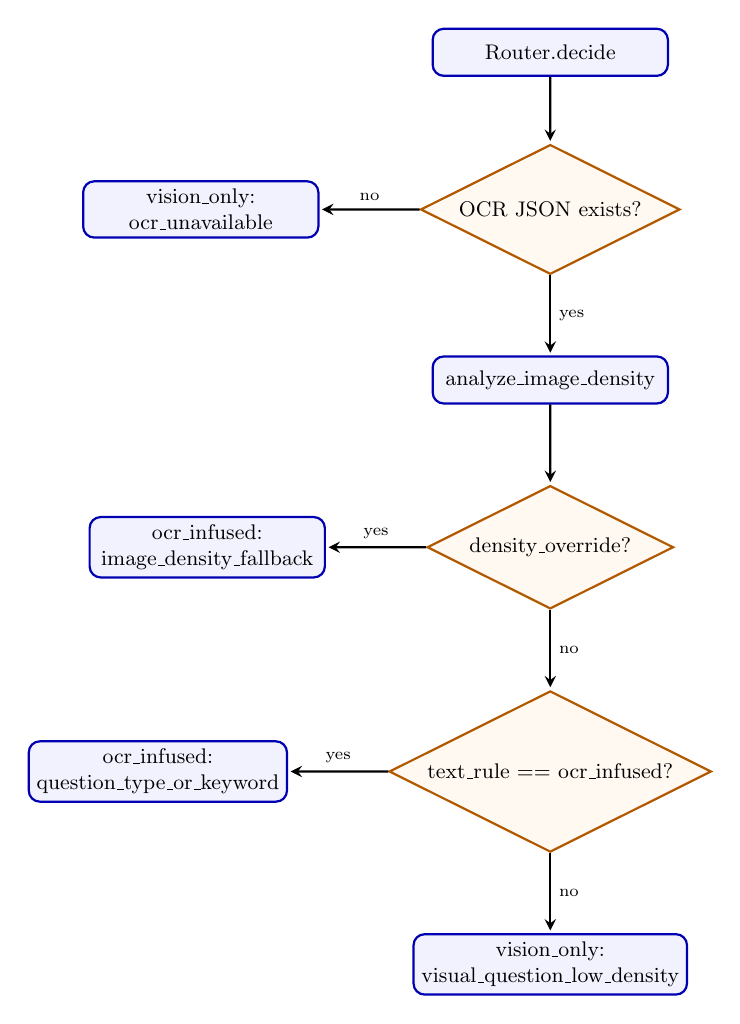
\begin{tikzpicture}[node distance=1.2cm and 1cm, >=stealth, thick, scale=0.85, every node/.style={transform shape}]
    \tikzset{
        block/.style={rectangle, draw=blue!70!black, fill=blue!5, rounded corners, minimum height=2em, minimum width=10em, align=center, font=\small},
        decision/.style={diamond, draw=orange!70!black, fill=orange!5, aspect=2, minimum width=10em, align=center, font=\small},
        line/.style={draw, ->, shorten >=1pt}
    }
    
    \node (Start) [block] {Router.decide};
    \node (OCRAvail) [decision, below=1cm of Start] {OCR JSON exists?};
    \node (Unavail) [block, left=1.5cm of OCRAvail] {vision\_only:\\ocr\_unavailable};
    \node (Density) [block, below=1.2cm of OCRAvail] {analyze\_image\_density};
    \node (Override) [decision, below=1.2cm of Density] {density\_override?};
    \node (InfusedD) [block, left=1.5cm of Override] {ocr\_infused:\\image\_density\_fallback};
    \node (TextCheck) [decision, below=1.2cm of Override] {text\_rule == ocr\_infused?};
    \node (InfusedT) [block, left=1.5cm of TextCheck] {ocr\_infused:\\question\_type\_or\_keyword};
    \node (Vision) [block, below=1.2cm of TextCheck] {vision\_only:\\visual\_question\_low\_density};
    
    \path [line] (Start) -- (OCRAvail);
    \path [line] (OCRAvail) -- node [above, font=\scriptsize] {no} (Unavail);
    \path [line] (OCRAvail) -- node [right, font=\scriptsize] {yes} (Density);
    \path [line] (Density) -- (Override);
    \path [line] (Override) -- node [above, font=\scriptsize] {yes} (InfusedD);
    \path [line] (Override) -- node [right, font=\scriptsize] {no} (TextCheck);
    \path [line] (TextCheck) -- node [above, font=\scriptsize] {yes} (InfusedT);
    \path [line] (TextCheck) -- node [right, font=\scriptsize] {no} (Vision);
    
\end{tikzpicture}
\caption{Routing Decision Tree}
\label{fig:routing_tree}
\end{figure}

\subsection{Stage A --- Text Rules (\texttt{\_text\_route})}
Applied to the question text and the \texttt{question\_types} list as defined in Table~\ref{tab:text_rules}.

\begin{table}[H]
\centering
\caption{Stage A --- Text Rules (\texttt{\_text\_route})}
\label{tab:text_rules}
\begin{tabular}{|p{10cm}|c|}
\hline
\textbf{Condition} & \textbf{Route} \\ \hline
\texttt{question\_types} intersect \texttt{LAYOUT\_HEAVY\_TYPES} & \texttt{ocr\_infused} \\ \hline
Question contains any \texttt{LAYOUT\_KEYWORDS} & \texttt{ocr\_infused} \\ \hline
\texttt{question\_types} intersect \texttt{OCR\_CAUTIOUS\_TYPES} AND layout keyword present & \texttt{ocr\_infused} \\ \hline
\texttt{question\_types} intersect \texttt{OCR\_CAUTIOUS\_TYPES} without layout keyword & \texttt{vision\_only} \\ \hline
Otherwise & \texttt{vision\_only} \\ \hline
\end{tabular}
\end{table}

\noindent\textbf{Constants (\texttt{config/settings.py}):}
\begin{itemize}
    \item \texttt{LAYOUT\_HEAVY\_TYPES}: \texttt{form}, \texttt{table/list}, \texttt{layout}, \texttt{handwritten}, \texttt{others}
    \item \texttt{VISUAL\_HEAVY\_TYPES} (eval cohort only): \texttt{figure/diagram}, \texttt{Image/Photo}, \texttt{Yes/No}, \texttt{free\_text}
    \item \texttt{OCR\_CAUTIOUS\_TYPES}: \texttt{figure/diagram}, \texttt{free\_text}
    \item \texttt{LAYOUT\_KEYWORDS}: \texttt{row}, \texttt{column}, \texttt{table}, \texttt{total}, \texttt{amount}, \texttt{sum}, \texttt{left}, \texttt{right}, \texttt{above}, \texttt{below}, \texttt{header}, \texttt{footer}, \texttt{field}, \texttt{box}
\end{itemize}

\subsection{Stage B --- Image Density Override (Pixel-Based)}
If text rules return \texttt{vision\_only}, the router may still force OCR when the image appears text-dense. This is implemented in \texttt{analyze\_image\_density()}:
\begin{enumerate}
    \item Convert the image to grayscale and optionally resize it to a maximum of 1024px.
    \item Compute \texttt{edge\_density} via Canny edge detection (OpenCV) or Sobel fallback.
    \item Compute a \texttt{low\_contrast\_flag} if pixel standard deviation is less than 35.0.
    \item Set \texttt{density\_override = True} if any of the following hold:
    \begin{itemize}
        \item \texttt{edge\_density > 0.18} (\texttt{DENSITY\_EDGE\_VERY\_HIGH})
        \item \texttt{edge\_density > 0.12} AND \texttt{low\_contrast\_flag} (\texttt{DENSITY\_EDGE\_THRESHOLD})
        \item \texttt{low\_contrast\_flag} AND \texttt{edge\_density > 0.08} (\texttt{DENSITY\_EDGE\_MID})
    \end{itemize}
\end{enumerate}
When \texttt{density\_override} is true, the route becomes \texttt{ocr\_infused} with the reason \texttt{image\_density\_fallback}.

\subsection{Hard Fallback}
If the OCR JSON file is missing for the document page, the route defaults to \texttt{vision\_only} with the reason \texttt{ocr\_unavailable}.

\subsection{Observed Routing Distribution (V2 Eval, n=200)}
Extracted from \texttt{baseline\_vs\_adaptive\_report.json} under \texttt{routing\_breakdown}, as shown in Table~\ref{tab:routing_dist}:

\begin{table}[H]
\centering
\caption{Observed Routing Distribution (V2 Eval, n=200)}
\label{tab:routing_dist}
\begin{tabular}{|l|c|c|}
\hline
\textbf{Final Routing Reason} & \textbf{Count} & \textbf{Mean ANLS} \\ \hline
\texttt{visual\_question\_low\_density} & 96 & 0.568 \\ \hline
\texttt{question\_type\_or\_keyword} & 84 & 0.756 \\ \hline
\texttt{low\_retrieval\_confidence} & 11 & 0.701 \\ \hline
\texttt{ocr\_empty\_after\_retrieval} & 6 & 0.647 \\ \hline
\texttt{image\_density\_fallback} & 3 & 0.667 \\ \hline
\end{tabular}
\end{table}

\textbf{Interpretation:} 96 out of 200 samples never entered the OCR retrieval path at the router. Out of the 104 that did, 84 successfully passed all gates and received OCR in the VLM prompt. The remainder fell back to vision-only after retrieval or gating failures.

\newpage
\section{Hybrid Retriever Agent}
\textbf{Implementation:} \texttt{src/agents/retriever\_agent.py}

The retriever selects a small subset of OCR lines (typically 50--150 per page) that are most relevant to the question.

\subsection{Hybrid Scoring Formula}
For each OCR line $i$, the hybrid score is calculated as follows:
\begin{align}
\text{sparse}_i &= \text{sparse\_match\_score}(\text{question}, \text{line}_i.\text{text}, \text{tokens}) \\
\text{dense}_i  &= \text{cosine\_similarity}(\text{embed}(\text{question}), \text{embed}(\text{window}_i)) \\
\text{final}_i  &= \alpha \cdot \text{dense}_i + (1 - \alpha) \cdot \text{sparse}_i
\end{align}

Table~\ref{tab:hybrid_params} defines the parameters used in the hybrid retriever.

\begin{table}[H]
\centering
\caption{Hybrid Scoring Formula Parameters}
\label{tab:hybrid_params}
\begin{tabular}{|p{6cm}|c|l|}
\hline
\textbf{Symbol / Metric} & \textbf{Value} & \textbf{Config Key} \\ \hline
$\alpha$ (Dense vs. sparse blend weight) & 0.7 & \texttt{HYBRID\_ALPHA} \\ \hline
Minimum score to retain line & 0.20 & \texttt{OCR\_MIN\_SCORE} \\ \hline
Top pool before budget & 40 & \texttt{OCR\_TOP\_K} \\ \hline
Max lines in output & 25 & \texttt{OCR\_MAX\_LINES} \\ \hline
Max characters (incl. coord overhead) & 1200 & \texttt{OCR\_MAX\_CHARS} \\ \hline
\end{tabular}
\end{table}

\noindent\textbf{Selection algorithm:}
\begin{enumerate}
    \item Score all lines; discard where $\text{final}_i < 0.20$.
    \item Sort by \texttt{(final\_score, label\_boost)} descending, where \texttt{label\_boost = 1} if \texttt{is\_label\_only(text)} else \texttt{0}.
    \item Take the top 40 into a candidate pool.
    \item Greedily add lines until the line count or character budget is exhausted (accounting for \texttt{len(text) + 30} per line for coordinate overhead).
\end{enumerate}

Figure~\ref{fig:hybrid_scoring} visualizes the retrieval scoring flow.

\begin{figure}[H]
\centering
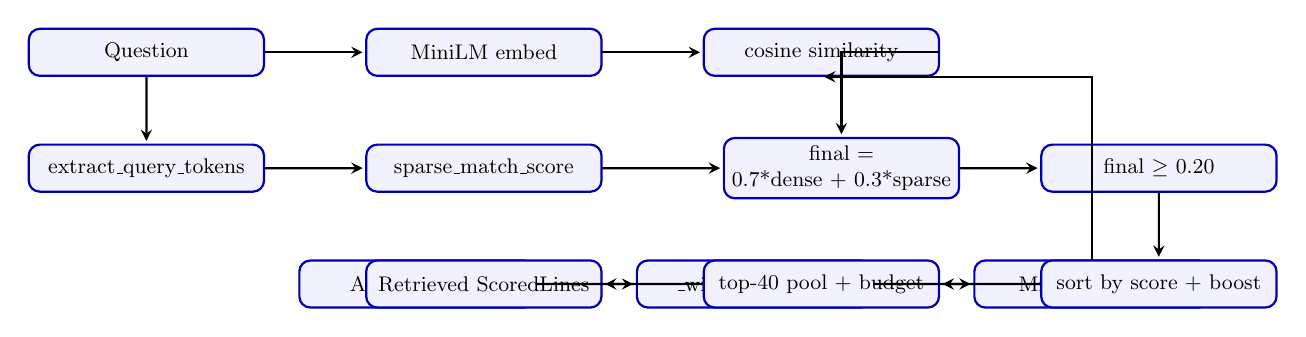
\begin{tikzpicture}[node distance=1cm and 0.8cm, >=stealth, thick, scale=0.85, every node/.style={transform shape}]
    \tikzset{
        block/.style={rectangle, draw=blue!70!black, fill=blue!5, rounded corners, minimum height=2em, minimum width=10em, align=center, font=\small},
        line/.style={draw, ->, shorten >=1pt}
    }
    
    \node (Q) [block] {Question};
    \node (Tokens) [block, below=1cm of Q] {extract\_query\_tokens};
    \node (DenseEmb) [block, right=1.5cm of Q] {MiniLM embed};
    
    \node (Lines) [block, below right=1cm and 0.5cm of Tokens] {All OCR lines};
    \node (Window) [block, right=1.5cm of Lines] {\_windowed\_texts};
    \node (LineEmb) [block, right=1.5cm of Window] {MiniLM embed};
    
    \node (Sparse) [block, right=1.5cm of Tokens] {sparse\_match\_score};
    \node (Cosine) [block, right=1.5cm of DenseEmb] {cosine similarity};
    
    \node (Blend) [block, right=1.8cm of Sparse] {final = \\ 0.7*dense + 0.3*sparse};
    
    \node (Filter) [block, right=1.2cm of Blend] {final $\ge$ 0.20};
    \node (Sort) [block, below=1cm of Filter] {sort by score + boost};
    \node (Budget) [block, left=1.5cm of Sort] {top-40 pool + budget};
    \node (Out) [block, left=1.5cm of Budget] {Retrieved ScoredLines};
    
    \path [line] (Q) -- (Tokens);
    \path [line] (Q) -- (DenseEmb);
    \path [line] (Lines) -- (Window);
    \path [line] (Window) -- (LineEmb);
    \path [line] (Tokens) -- (Sparse);
    \path [line] (DenseEmb) -- (Cosine);
    \path [line] (LineEmb) |- (Cosine.south);
    \path [line] (Sparse) -- (Blend);
    \path [line] (Cosine) -| (Blend.north);
    \path [line] (Blend) -- (Filter);
    \path [line] (Filter) -- (Sort);
    \path [line] (Sort) -- (Budget);
    \path [line] (Budget) -- (Out);
    
\end{tikzpicture}
\caption{Hybrid Scoring Formula and Selection Pipeline}
\label{fig:hybrid_scoring}
\end{figure}

\subsection{Dense Path --- sentence-transformers/all-MiniLM-L6-v2}
\textbf{Model:} \texttt{EMBEDDING\_MODEL = "sentence-transformers/all-MiniLM-L6-v2"} in \texttt{config/settings.py}.

\noindent\textbf{V2 Windowed Embeddings:} Instead of embedding isolated line text, each line is embedded as a 3-line context window:
\begin{equation}
\text{window}_i = \text{text}_{i-1} + \text{" "} + \text{text}_i + \text{" "} + \text{text}_{i+1}
\end{equation}
(boundary lines omit missing neighbors). This helper assists semantic matching when the answer text is spatially adjacent to a label (e.g., the question mentions ``college'' while the value line reads ``School of Public Health'' next to a ``College'' label).

\noindent\textbf{Caching:} Embeddings are stored at \texttt{data/cache/ocr\_embeddings/\{ucsf\_id\}\_\{page\_no\}\_w1.npz}. The suffix \texttt{\_w1} distinguishes V2 windowed caches from V1 isolated-line caches.

\noindent\textbf{Scoring:}
\begin{equation}
\text{dense}_i = \frac{q \cdot w_i}{\|q\| \cdot \|w_i\|}
\end{equation}
where $q$ is the question embedding and $w_i$ is the window embedding.

\noindent\textbf{Fallback:} If \texttt{sentence-transformers} is unavailable, character-level TF-IDF (3--5 grams) is used instead. Production/Kaggle runs should install \texttt{sentence-transformers} for consistent behavior.

\subsection{Sparse Path --- Keyword Extraction}
Keywords are extracted automatically from the question string, rather than being manually chosen per question. The flow is visualized in Figure~\ref{fig:keyword_flow}.

\begin{figure}[H]
\centering
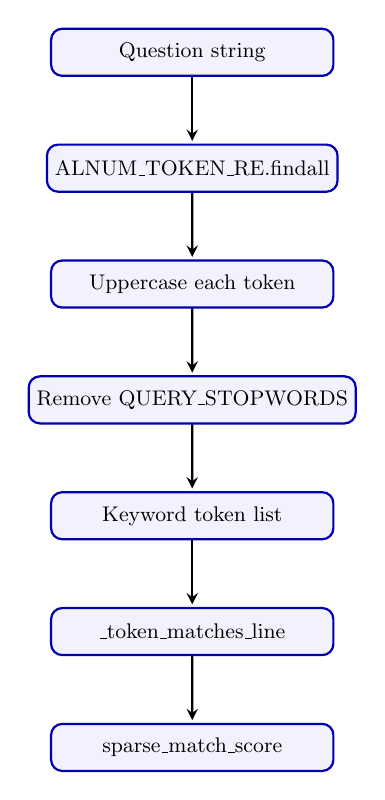
\begin{tikzpicture}[node distance=1.2cm and 1cm, >=stealth, thick, scale=0.85, every node/.style={transform shape}]
    \tikzset{
        block/.style={rectangle, draw=blue!70!black, fill=blue!5, rounded corners, minimum height=2em, minimum width=12em, align=center, font=\small},
        line/.style={draw, ->, shorten >=1pt}
    }
    
    \node (Q) [block] {Question string};
    \node (Regex) [block, below=1cm of Q] {ALNUM\_TOKEN\_RE.findall};
    \node (Upper) [block, below=1cm of Regex] {Uppercase each token};
    \node (Stop) [block, below=1cm of Upper] {Remove QUERY\_STOPWORDS};
    \node (Tokens) [block, below=1cm of Stop] {Keyword token list};
    \node (Match) [block, below=1cm of Tokens] {\_token\_matches\_line};
    \node (Score) [block, below=1cm of Match] {sparse\_match\_score};
    
    \path [line] (Q) -- (Regex);
    \path [line] (Regex) -- (Upper);
    \path [line] (Upper) -- (Stop);
    \path [line] (Stop) -- (Tokens);
    \path [line] (Tokens) -- (Match);
    \path [line] (Match) -- (Score);
    
\end{tikzpicture}
\caption{Sparse Path Keyword Extraction Flow}
\label{fig:keyword_flow}
\end{figure}

\noindent\textbf{Tokenization regex (\texttt{ALNUM\_TOKEN\_RE}):}
\begin{lstlisting}[language=Python]
\d+(?:\.\d+)?|[A-Za-z0-9]+(?:[-_/][A-Za-z0-9]+)*
\end{lstlisting}

\noindent\textbf{Stopwords removed (\texttt{QUERY\_STOPWORDS}, 18 tokens):} \\
\texttt{A, AN, AND, ARE, AT, FOR, IN, IS, OF, ON, OR, THE, TO, WAS, WHAT, WHICH, WHO, WHOM}

\noindent\textbf{Examples:} Table~\ref{tab:stopword_examples} provides examples of stopword filtering on questions.

\begin{table}[H]
\centering
\caption{Sparse Path Stopword Filtering Examples}
\label{tab:stopword_examples}
\begin{tabular}{|p{6cm}|p{4cm}|p{5cm}|}
\hline
\textbf{Question} & \textbf{Raw Tokens} & \textbf{After Stopword Filter} \\ \hline
\texttt{"What is the specimen ?"} & What, is, the, specimen & \texttt{SPECIMEN} \\ \hline
\texttt{"Which is the college?"} & Which, is, the, college & \texttt{COLLEGE} \\ \hline
\texttt{"What is the date on which the request for change was prepared?"} & What, is, the, date, on, which, the, request, for, change, was, prepared & \texttt{DATE, REQUEST, CHANGE, PREPARED} \\ \hline
\end{tabular}
\end{table}

\noindent\textbf{Sparse score computation:}
\begin{equation}
\text{score} = \frac{\text{matched\_keywords}}{\text{total\_keywords}}
\end{equation}
If any keyword with length $\ge 3$ matches the line, the score is set to $1.0$ (early return).

\noindent\textbf{Match rules (\texttt{\_token\_matches\_line}):}
\begin{itemize}
    \item If the keyword $\in$ \texttt{FIELD\_LABEL\_KEYWORDS}: whole-word boundary match \texttt{\textbackslash bTOKEN\textbackslash b}.
    \item Otherwise: substring match in uppercased line text.
\end{itemize}

\noindent\textbf{Field label keywords (\texttt{FIELD\_LABEL\_KEYWORDS}):} \\
\texttt{COLLEGE, NAME, SPECIMEN, TYPE, ID, NO, DATE, ADDRESS, PHONE, EMAIL, DEPARTMENT, SCHOOL, TITLE}

\subsection{V2 Retriever Fixes (Implementation Rationale)}
Table~\ref{tab:retriever_fixes} details the changes made in the V2 retriever.

\begin{table}[H]
\centering
\caption{V2 Retriever Fixes (Implementation Rationale)}
\label{tab:retriever_fixes}
\begin{tabular}{|p{5cm}|p{5cm}|p{5cm}|}
\hline
\textbf{V1 Issue} & \textbf{V2 Fix} & \textbf{Effect} \\ \hline
Token \texttt{THE} triggered sparse=1.0 on most lines & \texttt{QUERY\_STOPWORDS} filter & Stops retrieval pool pollution \\ \hline
Label lines penalized \texttt{final *= 0.5} & Penalty removed & Labels can rank high and become expansion anchors \\ \hline
Isolated line embeddings & Windowed dense \texttt{\_w1} & Neighbor-aware semantic matching \\ \hline
Tie at sparse=1.0 & Prefer \texttt{is\_label\_only} lines in sort & Short field labels beat long descriptive lines \\ \hline
\end{tabular}
\end{table}

\newpage
\section{Context Expander --- Spatial Neighbor Logic}
\textbf{Implementation:} \texttt{src/agents/context\_expander.py} \\
\textbf{Enabled by:} \texttt{ENABLE\_CONTEXT\_EXPANSION = True} in \texttt{config/settings.py}

The retriever may return a field \textbf{label} (e.g., \texttt{"Specimen:"}) without the \textbf{value} (e.g., \texttt{"10 rat sera"}) on the line below. The expander uses bounding-box geometry to add spatially related lines.

\subsection{Spatial Rules}
For each retrieved anchor with bounding box \texttt{[x1, y1, x2, y2]}, the expansion logic applies the rules shown in Figure~\ref{fig:spatial_rules}.

\begin{figure}[H]
\centering
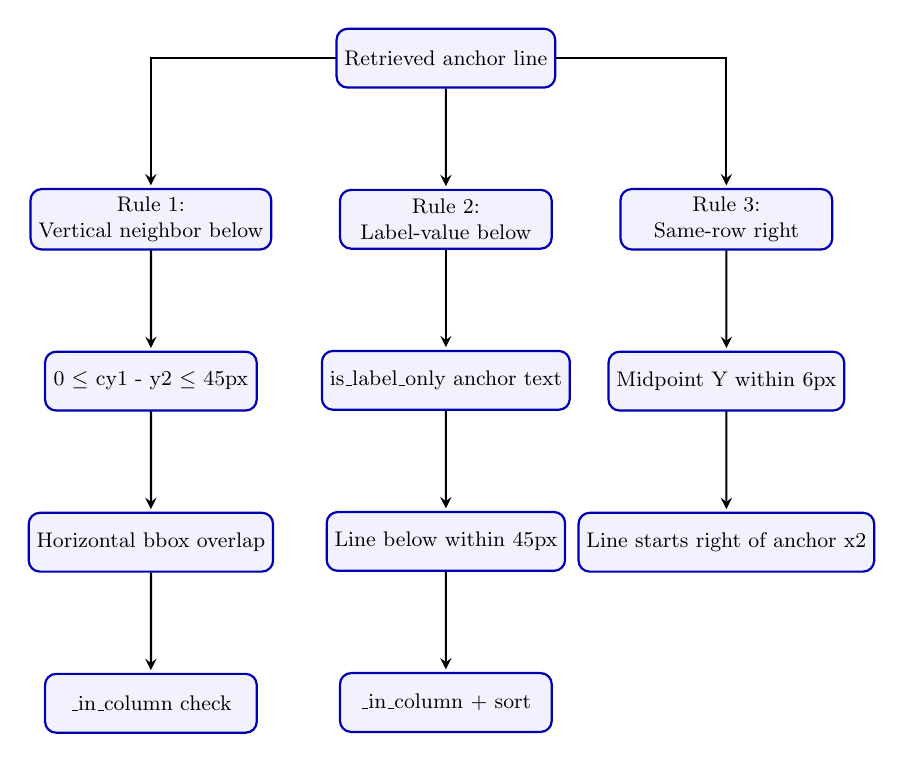
\begin{tikzpicture}[node distance=1.5cm and 1cm, >=stealth, thick, scale=0.85, every node/.style={transform shape}]
    \tikzset{
        block/.style={rectangle, draw=blue!70!black, fill=blue!5, rounded corners, minimum height=2.5em, minimum width=9em, align=center, font=\small},
        line/.style={draw, ->, shorten >=1pt}
    }
    
    \node (Anchor) [block] {Retrieved anchor line};
    
    \node (Rule2) [block, below=of Anchor] {Rule 2:\\Label-value below};
    \node (Rule1) [block, left=of Rule2] {Rule 1:\\Vertical neighbor below};
    \node (Rule3) [block, right=of Rule2] {Rule 3:\\Same-row right};
    
    \node (G1) [block, below=of Rule1] {0 $\le$ cy1 - y2 $\le$ 45px};
    \node (G2) [block, below=of G1] {Horizontal bbox overlap};
    \node (G3) [block, below=of G2] {\_in\_column check};
    
    \node (L1) [block, below=of Rule2] {is\_label\_only anchor text};
    \node (L2) [block, below=of L1] {Line below within 45px};
    \node (L3) [block, below=of L2] {\_in\_column + sort};
    
    \node (R1) [block, below=of Rule3] {Midpoint Y within 6px};
    \node (R2) [block, below=of R1] {Line starts right of anchor x2};
    
    \path [line] (Anchor) -| (Rule1);
    \path [line] (Anchor) -- (Rule2);
    \path [line] (Anchor) -| (Rule3);
    
    \path [line] (Rule1) -- (G1);
    \path [line] (G1) -- (G2);
    \path [line] (G2) -- (G3);
    
    \path [line] (Rule2) -- (L1);
    \path [line] (L1) -- (L2);
    \path [line] (L2) -- (L3);
    
    \path [line] (Rule3) -- (R1);
    \path [line] (R1) -- (R2);
    
\end{tikzpicture}
\caption{Spatial Rules for Context Expansion}
\label{fig:spatial_rules}
\end{figure}

The geometric constraints and V2 parameters are detailed in Table~\ref{tab:spatial_rules_table}.

\begin{table}[H]
\centering
\caption{Spatial Rules for Context Expansion}
\label{tab:spatial_rules_table}
\begin{tabular}{|p{4.5cm}|p{5.5cm}|p{5cm}|}
\hline
\textbf{Rule} & \textbf{Geometry} & \textbf{V2 Parameters} \\ \hline
Vertical neighbor below & Gap $0 \le \text{cy1} - \text{y2} \le 45$ px, x-overlap & + \texttt{\_in\_column()} \\ \hline
Label $\rightarrow$ value below & Anchor is label-only; nearest line below in same column & Sort: \texttt{(abs(ln.x1 - x1), ln.y1)} \\ \hline
Same-row right & Vertical midpoints within 6 px; \texttt{ln.x1 > x2} & \texttt{Y\_OVERLAP\_TOLERANCE = 6} \\ \hline
\end{tabular}
\end{table}

\noindent\textbf{Column filter (\texttt{\_in\_column}):} A candidate bounding box must overlap the anchor's x-range extended by \texttt{COLUMN\_X\_PAD = 20} px:
\begin{equation}
\text{candidate.x1} \le \text{anchor.x2} + \text{pad} \quad \text{AND} \quad \text{candidate.x2} \ge \text{anchor.x1} - \text{pad}
\end{equation}

\noindent\textbf{Label detection (\texttt{is\_label\_only}) --- V2:}
\begin{enumerate}
    \item Matches \texttt{LABEL\_ONLY\_RE} (e.g., \texttt{"College:"}).
    \item OR trailing colon with empty value (e.g., \texttt{"Name: "}).
    \item OR short text ($< 40$ chars) matching the \texttt{FIELD\_LABEL\_KEYWORDS} prefix (e.g., \texttt{"College"}, \texttt{"Specimen"}).
\end{enumerate}

\noindent\textbf{Inherited score for expanded lines:}
\begin{equation}
\text{expanded.final\_score} = \text{anchor.final\_score} \times 0.9
\end{equation}

\subsection{Post-Expansion Budget and Ordering (V2)}
After all expansion rules execute, the function \texttt{\_apply\_expansion\_budget()} performs:
\begin{enumerate}
    \item \textbf{Always retains} all original retrieved anchor lines.
    \item Adds highest-scoring expanded neighbors until reaching \texttt{OCR\_MAX\_LINES} (25) or \texttt{OCR\_MAX\_CHARS} (1200).
    \item Sorts the final set by \texttt{(bbox.y1, bbox.x1)} to reflect the document's natural reading order.
\end{enumerate}

\subsection{Worked Example --- Specimen Question (V2 Eval)}
\begin{itemize}
    \item \textbf{Question:} \texttt{"What is the specimen ?"} (question\_id 19005)
    \item \textbf{Retrieved line\_ids:} \texttt{[22, 21, 20, 85, 83, 4]}
    \item \textbf{Expanded line\_ids:} \texttt{[4, 8, 20, 23, 21, 22, 24, 25, 83, 85]} (neighbors 8, 23, 24, 25 added)
    \item \textbf{Top final\_score:} 0.497 (passed gate $\ge$ 0.45)
    \item \textbf{Predicted answer:} \texttt{"10 rat sera"} --- \textbf{ANLS 1.0}, \texttt{used\_ocr: true}
\end{itemize}
Expansion attached the value line that sparse retrieval alone might miss because the keyword \texttt{SPECIMEN} matched the label, not the answer text.

\newpage
\section{Formatter and OCR Prompt Infusion}
\textbf{Formatter:} \texttt{src/agents/formatter\_agent.py} \\
\textbf{Sanitizer:} \texttt{src/agents/text\_sanitizer.py} \\
\textbf{Prompt assembly:} \texttt{src/models/inference.py} $\rightarrow$ \texttt{\_build\_prompt()}

\subsection{Sanitization}
Before formatting, each line passes through \texttt{sanitize\_line\_text()}:
\begin{itemize}
    \item Drop empty lines.
    \item Drop lines starting with boilerplate: \texttt{INSTRUCTION}, \texttt{NOTICE}, \texttt{USER} (\texttt{OCR\_BOILERPLATE\_DENYLIST}).
    \item Normalize \texttt{::} $\rightarrow$ \texttt{:}.
    \item Strip leading \texttt{\#} characters (form markers that hijacked V1 predictions).
\end{itemize}
Lines returning \texttt{None} are excluded from the snippet.

\subsection{Layout-Preserving Format}
After sanitization, lines are sorted by reading order: \texttt{(bbox[1], bbox[0])} (top-to-bottom, then left-to-right). Each line is formatted as:
\begin{lstlisting}
[x1,y1,x2,y2] line_text
\end{lstlisting}

\noindent\textbf{Example snippet block:}
\begin{lstlisting}
[440,805,753,837] Specimen:
[445,842,620,870] 10 rat sera
[1214,254,1539,287] INSTRUCTION FOR USER
\end{lstlisting}
(The third line would be dropped by the sanitizer in practice.)

\subsection{VLM Prompt Structure (XML Wrapper)}
When \texttt{used\_ocr=true}, \texttt{\_build\_prompt()} constructs the following string prompt:
\begin{lstlisting}[language=XML]
<|user|>
<|image_1|>
Answer briefly with only the exact value or phrase from the document. Do not use full sentences.
<document_ocr_context>
OCR hints (may be incomplete; prefer the image if hints lack the answer):
[x1,y1,x2,y2] line1
[x1,y1,x2,y2] line2
</document_ocr_context>
Question: {question}<|end|>
<|assistant|>
\end{lstlisting}

\noindent\textbf{Multimodal inference:} \texttt{processor(text=prompt, images=image)} --- the image token \texttt{<|image\_1|>} is \textbf{always} present. OCR text is supplementary context, not a replacement for vision.

\noindent\textbf{Disclaimer (\texttt{OCR\_DISCLAIMER}):} Instructs the model that OCR may be incomplete and to prefer the image when hints lack the answer.

\noindent\textbf{Generation controls:}
\begin{itemize}
    \item \texttt{DOCVQA\_MAX\_NEW\_TOKENS = 20} --- short answers only.
    \item \texttt{DOCVQA\_STOP\_STRINGS} --- stop on \texttt{\textbackslash n}, \texttt{\#}, \texttt{<|user|>}, \texttt{<document\_ocr\_context>} to prevent runaway or boilerplate copying.
    \item \texttt{do\_sample=False} --- deterministic greedy decoding.
\end{itemize}

\noindent\textbf{Audit metadata:} \texttt{prompt\_meta.used\_xml\_wrapper = true}, \texttt{prompt\_meta.ocr\_in\_prompt = true} when the quality gate passes.

\newpage
\section{Quality Gate}
\textbf{Implementation:} \texttt{src/agents/quality\_gate.py}

The gate is the final safety check before OCR enters the VLM prompt. \textbf{All three checks must pass.}

\subsection{Check 1 --- Top Retrieval Confidence}
\begin{equation}
\max_{s \in \text{scored\_anchors}} \text{s.final\_score} \ge \text{OCR\_GATE\_MIN\_SCORE} \ (0.45)
\end{equation}
Uses scores from \textbf{retrieved anchor lines only} (before expansion neighbor inheritance). This ensures at least one line was confidently matched to the question.

\subsection{Check 2 --- Information Gain}
\begin{align}
\text{snippet\_tokens} &= \text{extract\_query\_tokens}(\text{formatted.text\_block}) \\
\text{new\_tokens}     &= \text{snippet\_tokens} \setminus \text{question\_tokens}
\end{align}
\textbf{FAIL if:} \texttt{new\_tokens} is empty AND \texttt{len(snippet\_tokens)} $\le$ \texttt{len(question\_tokens)}. \\
The snippet must contribute tokens beyond what the question already contains. This prevents injecting OCR that merely repeats the question wording without introducing answer content.

\subsection{Check 3 --- Label-Value Content (Conditional)}
Applies only when the question matches \texttt{\textbackslash bwhat is\textbackslash b} or \texttt{\textbackslash bwhat are\textbackslash b}:
The snippet must contain answer-like content:
\begin{itemize}
    \item A line with \texttt{Label: value} where value is non-empty alphanumeric, OR
    \item A non-label line with at least 2 alphanumeric characters.
\end{itemize}

\subsection{Gate Failure Behavior}
If any check fails:
\begin{itemize}
    \item \texttt{routing.route} is overwritten to \texttt{vision\_only}.
    \item \texttt{routing.reason = "low\_retrieval\_confidence"}.
    \item \texttt{used\_ocr = false}.
    \item The VLM receives the image + question only (identical to baseline prompt structure).
\end{itemize}

\noindent\textbf{Example --- Eastern Airlines (gate failure, vision success):}
\begin{itemize}
    \item \textbf{Question:} \texttt{"What is the name of the issuing airlines?"}
    \item \textbf{Top score:} $\approx 0.303$ ($< 0.45$) $\rightarrow$ gate failed.
    \item \textbf{used\_ocr:} \texttt{false} $\rightarrow$ VLM used vision only.
    \item \textbf{Predicted:} \texttt{"Eastern Airlines"} --- \textbf{ANLS 1.0}.
\end{itemize}
Injecting low-confidence OCR would likely have hurt accuracy.

\newpage
\section{V2 Improvements Summary --- Design Intent vs. Implementation}
Table~\ref{tab:v2_improvements} summarizes the comparison between V1 issues and V2 solutions.

\begin{table}[H]
\centering
\caption{V2 Improvements Summary --- Design Intent vs. Implementation}
\label{tab:v2_improvements}
\begin{small}
\begin{tabular}{|p{4cm}|p{4cm}|p{3.5cm}|p{3.5cm}|}
\hline
\textbf{Design Problem (V1)} & \textbf{V2 Implementation} & \textbf{Source File} & \textbf{Expected ANLS Effect} \\ \hline
Stopword \texttt{THE} caused sparse=1.0 everywhere & \texttt{QUERY\_STOPWORDS} + boundary matching for field keywords & \texttt{retriever\_agent.py}, \texttt{settings.py} & Less retrieval noise; cleaner snippets \\ \hline
Label penalty prevented spatial expansion & Removed \texttt{final *= 0.5} on label lines & \texttt{retriever\_agent.py} & Label$\rightarrow$value chains activate \\ \hline
Fine-print labels missed (\texttt{College} without colon) & \texttt{FIELD\_LABEL\_KEYWORDS} in \texttt{is\_label\_only()} & \texttt{context\_expander.py} & Form field expansion works \\ \hline
Multi-column forms picked wrong neighbor & \texttt{\_in\_column()} + column-first sort & \texttt{context\_expander.py} & Correct column values retrieved \\ \hline
Unbounded expansion overflowed prompt & \texttt{\_apply\_expansion\_budget()} & \texttt{context\_expander.py} & Stable prompt size \\ \hline
Isolated embeddings missed adjacent answers & Windowed dense + \texttt{\_w1} cache suffix & \texttt{retriever\_agent.py} & Better semantic match on values \\ \hline
Skewed OCR boxes broke row alignment & Midpoint \texttt{\_y\_overlap} (6 px tolerance) & \texttt{context\_expander.py} & Same-row field detection \\ \hline
\end{tabular}
\end{small}
\end{table}

\section{Evaluation Methodology}

\subsection{Evaluation Protocol}
The baseline and V2 evaluation streams are structured as shown in Figure~\ref{fig:eval_protocol}.

\begin{figure}[H]
\centering
\begin{tikzpicture}[node distance=1.2cm and 1cm, >=stealth, thick, scale=0.85, every node/.style={transform shape}]
    \tikzset{
        block/.style={rectangle, draw=blue!70!black, fill=blue!5, rounded corners, minimum height=2.5em, minimum width=14em, align=center, font=\small},
        line/.style={draw, ->, shorten >=1pt}
    }
    
    \node (Subset) [block] {eval\_subset\_200.json\\(200 samples, seed=42)};
    
    \node (Baseline) [block, below left=1.5cm and 0.5cm of Subset] {chunked\_evaluation\\-{}-mode baseline};
    \node (Adaptive) [block, below right=1.5cm and 0.5cm of Subset] {chunked\_evaluation\\-{}-mode ocr\_adaptive\\-{}-version v2};
    
    \node (BOut) [block, below=of Baseline] {baseline\_200/\\results\_merged.json};
    \node (AOut) [block, below=of Adaptive] {ocr\_adaptive\_200\_v2/\\results\_merged.json};
    
    \node (Compare) [block, below=2cm of ($(BOut.south)!0.5!(AOut.south)$)] {compare\_baselines.py\\-{}-adaptive-version v2};
    \node (Report) [block, below=of Compare] {comparisons/\\baseline\_vs\_adaptive\_report.json};
    
    \path [line] (Subset) -| (Baseline);
    \path [line] (Subset) -| (Adaptive);
    \path [line] (Baseline) -- (BOut);
    \path [line] (Adaptive) -- (AOut);
    \path [line] (BOut) |- (Compare);
    \path [line] (AOut) |- (Compare);
    \path [line] (Compare) -- (Report);
    
\end{tikzpicture}
\caption{Evaluation Protocol}
\label{fig:eval_protocol}
\end{figure}

Table~\ref{tab:eval_scripts} outlines the roles of the evaluation scripts.

\begin{table}[H]
\centering
\caption{Evaluation Scripts}
\label{tab:eval_scripts}
\begin{tabular}{|l|p{10cm}|}
\hline
\textbf{Script} & \textbf{Purpose} \\ \hline
\texttt{scripts/build\_eval\_subset.py} & Build 200-sample stratified subset \\ \hline
\texttt{scripts/chunked\_evaluation.py} & Run inference in 10 chunks $\times$ 20 samples \\ \hline
\texttt{scripts/compare\_baselines.py} & Paired ANLS comparison \\ \hline
\texttt{scripts/ablation\_report.py} & Damage cases, hijacking analysis \\ \hline
\end{tabular}
\end{table}

\noindent\textbf{Hardware:} Kaggle T4 GPU; Phi-3.5-Vision float16; \texttt{sentence-transformers} for dense retrieval.

\subsection{Stratified Subset --- Two Cohorts}
Built by \texttt{scripts/build\_eval\_subset.py} from SP-DocVQA validation annotations, as shown in Table~\ref{tab:stratified_cohorts}:

\begin{table}[H]
\centering
\caption{Stratified Subset Cohorts}
\label{tab:stratified_cohorts}
\begin{tabular}{|l|c|p{8cm}|}
\hline
\textbf{Cohort} & \textbf{Count} & \textbf{Assignment Rule} \\ \hline
\texttt{layout\_heavy} & 100 & Primary \texttt{question\_type} in \texttt{LAYOUT\_HEAVY\_TYPES} \\ \hline
\texttt{visual\_heavy} & 100 & Primary \texttt{question\_type} in \texttt{VISUAL\_HEAVY\_TYPES} \\ \hline
\end{tabular}
\end{table}

\textbf{Important:} Cohort labels come from \textbf{DocVQA question type annotations}, not from image classification. They are used for \textbf{eval reporting breakdown}, not directly by the router (router uses the same \texttt{question\_types} list but applies different logic). Random seed: \texttt{EVAL\_SUBSET\_SEED = 42} for reproducibility.

\subsection{Paired Comparison Design}
\begin{itemize}
    \item \textbf{Same 200 question\_ids} evaluated under both modes.
    \item \textbf{Same VLM} (Phi-3.5-Vision-Instruct), same decoding settings.
    \item \textbf{Only difference:} Baseline prompt has no \texttt{<document\_ocr\_context>} block; V2 adaptive adds it when \texttt{used\_ocr=true}.
    \item Per-sample ANLS computed independently; mean ANLS = average over 200 samples.
\end{itemize}

\subsection{Fairness Controls}
\begin{itemize}
    \item Baseline never receives OCR hints (mode enforced in \texttt{\_build\_prompt}).
    \item Adaptive falls back to baseline-equivalent prompt when gate fails (\texttt{used\_ocr=false}).
    \item OCR JSON is identical for both modes (pre-extracted Azure output).
    \item Chunked evaluation with resume prevents partial-run bias.
\end{itemize}

\newpage
\section{ANLS Metric --- Definition and Implementation}
\textbf{Implementation:} \texttt{src/utils/metrics.py} \\
\textbf{Threshold:} \texttt{ANLS\_THRESHOLD = 0.5} (default in \texttt{anls\_score()})

\subsection{Per-Sample ANLS Formula}
For prediction $p$ and each ground-truth answer $g$:

\noindent\textbf{Step 1 --- Normalize text (\texttt{\_normalize\_text}):}
\begin{itemize}
    \item Lowercase.
    \item Remove articles: \texttt{a}, \texttt{an}, \texttt{the}.
    \item Remove punctuation.
    \item Collapse whitespace.
\end{itemize}

\noindent\textbf{Step 2 --- Normalized Levenshtein similarity:}
\begin{equation}
\text{similarity}(p, g) = 1 - \frac{\text{edit\_distance}(p, g)}{\max(|p|, |g|)}
\end{equation}

\noindent\textbf{Step 3 --- Apply ANLS threshold:}
\begin{equation}
\text{ANLS}(p, g) = \begin{cases} 
0 & \text{if } \text{similarity}(p, g) < 0.5 \\ 
\frac{\text{similarity}(p, g) - 0.5}{1 - 0.5} & \text{otherwise} 
\end{cases}
\end{equation}

\noindent\textbf{Step 4 --- Multiple ground truths:}
\begin{equation}
\text{ANLS\_sample} = \max_{g \in \text{ground\_truths}} \text{ANLS}(p, g)
\end{equation}

\subsection{Dataset-Level Metrics}
\begin{equation}
\text{mean\_ANLS} = \frac{1}{N} \sum_{i=1}^N \text{ANLS\_sample}_i \quad (N = 200)
\end{equation}
\begin{equation}
\text{exact\_match} = \frac{1}{N} \sum_{i=1}^N \mathbb{I}(\text{normalize}(p_i) == \text{normalize}(g_i))
\end{equation}

\subsection{Worked Examples}
Table~\ref{tab:anls_worked_examples} displays how specific predictions match target ground truths under ANLS.

\begin{table}[H]
\centering
\caption{ANLS Worked Examples}
\label{tab:anls_worked_examples}
\begin{tabular}{|l|l|c|c|}
\hline
\textbf{Prediction} & \textbf{Ground Truth} & \textbf{Similarity} & \textbf{ANLS} \\ \hline
\texttt{"10 rat sera"} & \texttt{"10 rat sera"} & 1.0 & \textbf{1.0} \\ \hline
\texttt{"JOHN SMITH"} & \texttt{"John Smith"} & 1.0 & \textbf{1.0} \\ \hline
\texttt{"8/25/86"} & \texttt{"8/25/88"} & $\approx$ 0.86 & \textbf{(0.86$-$0.5)/0.5 = 0.72} \\ \hline
\texttt{"8/25/15"} & \texttt{"8/25/88"} & $\approx$ 0.71 & \textbf{(0.71$-$0.5)/0.5 = 0.43} \\ \hline
\texttt{"xyz"} & \texttt{"abc"} & low & \textbf{0.0} \\ \hline
\end{tabular}
\end{table}

ANLS rewards near-matches above 50\% character similarity and zeroes out poor matches.

\newpage
\section{Results and Evidence of Improvement}

\subsection{Overall Performance}
Table~\ref{tab:overall_perf} outlines the overall performance comparison.

\begin{table}[H]
\centering
\caption{Overall Performance comparison}
\label{tab:overall_perf}
\begin{tabular}{|l|c|c|}
\hline
\textbf{Metric} & \textbf{Baseline} & \textbf{V2 Adaptive} \\ \hline
Mean ANLS & 0.506 & \textbf{0.658} \\ \hline
Exact match & 0.420 & \textbf{0.595} \\ \hline
Samples & 200 & 200 \\ \hline
\end{tabular}
\end{table}
\textbf{Absolute improvement: +0.152 mean ANLS (+30\% relative).}

\subsection{By Eval Cohort}
Table~\ref{tab:cohort_perf} shows the breakdown of performance across cohorts.

\begin{table}[H]
\centering
\caption{Performance by Evaluation Cohort}
\label{tab:cohort_perf}
\begin{tabular}{|l|c|c|c|}
\hline
\textbf{Cohort} & \textbf{Baseline ANLS} & \textbf{V2 ANLS} & \textbf{Delta} \\ \hline
Layout-heavy (n=100) & 0.568 & 0.770 & \textbf{+0.202} \\ \hline
Visual-heavy (n=100) & 0.444 & 0.546 & \textbf{+0.102} \\ \hline
\end{tabular}
\end{table}
The largest gains occurred on layout-heavy documents where OCR infusion targets forms, tables, and structured fields.

\subsection{By Question Type (Selected)}
Table~\ref{tab:qtype_perf} showcases performance breakdown by specific question types.

\begin{table}[H]
\centering
\caption{Performance by Question Type}
\label{tab:qtype_perf}
\begin{tabular}{|l|c|c|c|}
\hline
\textbf{Question Type} & \textbf{Baseline} & \textbf{V2} & \textbf{Delta} \\ \hline
form & 0.603 & 0.790 & +0.187 \\ \hline
table/list & 0.376 & 0.771 & +0.395 \\ \hline
layout & 0.571 & 0.800 & +0.229 \\ \hline
handwritten & 0.521 & 0.683 & +0.162 \\ \hline
figure/diagram & 0.435 & 0.584 & +0.149 \\ \hline
free\_text & 0.457 & 0.554 & +0.097 \\ \hline
\end{tabular}
\end{table}

\subsection{Per-Sample Win/Tie Analysis}
Table~\ref{tab:wintie_analysis} presents the win/loss breakdown across the 200 samples.

\begin{table}[H]
\centering
\caption{Per-Sample Win/Tie Analysis}
\label{tab:wintie_analysis}
\begin{tabular}{|l|c|}
\hline
\textbf{Outcome} & \textbf{Count} \\ \hline
V2 adaptive wins (higher ANLS) & 46 \\ \hline
Baseline wins & 6 \\ \hline
Tie (identical ANLS) & 148 \\ \hline
\end{tabular}
\end{table}
Adaptive wins outnumber baseline wins 46:6, demonstrating improvement is not driven by a handful of outliers.

\subsection{Success Case --- Specimen (question\_id 19005)}
\begin{itemize}
    \item \textbf{Question:} \texttt{"What is the specimen ?"}
    \item \textbf{Routing:} \texttt{question\_type\_or\_keyword} $\rightarrow$ OCR infused
    \item \textbf{Retrieval + expansion} included value line.
    \item \textbf{used\_ocr:} \texttt{true}
    \item \textbf{Prediction:} \texttt{"10 rat sera"} --- \textbf{ANLS 1.0}
\end{itemize}
This demonstrates the end-to-end pipeline: router $\rightarrow$ hybrid retrieval $\rightarrow$ spatial expansion $\rightarrow$ quality gate $\rightarrow$ VLM with OCR hints.

\subsection{Honest Failure Case --- Date (question\_id 18964)}
\begin{itemize}
    \item \textbf{Question:} \texttt{"What is the date on which the request for change was prepared?"}
    \item \textbf{Ground truth:} \texttt{"8/25/88"}
    \item \textbf{Baseline (vision only):} \texttt{"8/25/86"} --- ANLS $\approx$ 0.72
    \item \textbf{V2 adaptive (\texttt{used\_ocr: true}):} \texttt{"8/25/15"} --- ANLS $\approx$ 0.43
\end{itemize}
Azure OCR misread the handwritten year. The VLM copied bad OCR text from the snippet instead of correcting from the image. This demonstrates:
\begin{enumerate}
    \item The VLM \textbf{is} being used (it generated the string).
    \item OCR infusion can \textbf{hurt} when OCR errors occur.
    \item The quality gate checks retrieval confidence, not OCR correctness against ground truth (ground truth is unavailable at inference time).
\end{enumerate}

\subsection{Limitations}
\begin{enumerate}
    \item \textbf{Cohort labels} derive from DocVQA metadata, not automatic image classification.
    \item \textbf{Production deployment} would lack \texttt{question\_types}; router must rely on question keywords + image density.
    \item \textbf{OCR quality ceiling} --- Azure OCR errors propagate when the VLM trusts hints.
    \item \textbf{148 ties} --- many samples unchanged between modes; improvement concentrated where OCR helps.
    \item \textbf{No fine-tuning} --- Phi-3.5 weights are frozen; all gains from inference-time retrieval.
\end{enumerate}

\newpage
\section{Implementation Traceability Appendix}
Table~\ref{tab:traceability} maps report sections to the corresponding source code locations.

\begin{table}[H]
\centering
\caption{Implementation Traceability Appendix}
\label{tab:traceability}
\begin{small}
\begin{tabular}{|p{4.5cm}|p{4.5cm}|p{6cm}|}
\hline
\textbf{Report Section} & \textbf{Source File} & \textbf{Key Constants / Functions} \\ \hline
Pipeline orchestration & \texttt{src/agents/pipeline.py} & \texttt{AgenticDocVQAPipeline.prepare()} \\ \hline
Router & \texttt{src/agents/router\_agent.py} & \texttt{\_text\_route()}, \texttt{RouterAgent.decide()} \\ \hline
Image density & \texttt{src/agents/image\_density.py} & \texttt{analyze\_image\_density()}, \texttt{density\_override} \\ \hline
Hybrid retriever & \texttt{src/agents/retriever\_agent.py} & \texttt{extract\_query\_tokens()}, \texttt{HybridRetrieverAgent.retrieve()} \\ \hline
Context expander & \texttt{src/agents/context\_expander.py} & \texttt{expand\_context()}, \texttt{is\_label\_only()}, \texttt{\_in\_column()} \\ \hline
Formatter & \texttt{src/agents/formatter\_agent.py} & \texttt{LayoutFormatterAgent.format()} \\ \hline
Sanitizer & \texttt{src/agents/text\_sanitizer.py} & \texttt{sanitize\_line\_text()} \\ \hline
Quality gate & \texttt{src/agents/quality\_gate.py} & \texttt{passes\_quality\_gate()} \\ \hline
VLM inference & \texttt{src/models/inference.py} & \texttt{\_build\_prompt()}, \texttt{generate\_answer()}, \texttt{evaluate()} \\ \hline
OCR loading & \texttt{src/data/ocr\_loader.py} & \texttt{load\_ocr\_lines()}, \texttt{OcrLine} \\ \hline
Metrics & \texttt{src/utils/metrics.py} & \texttt{anls\_score()}, \texttt{calculate\_metrics()} \\ \hline
Configuration & \texttt{config/settings.py} & All \texttt{OCR\_*}, \texttt{HYBRID\_ALPHA}, \texttt{QUERY\_STOPWORDS}, etc. \\ \hline
Eval subset & \texttt{scripts/build\_eval\_subset.py} & \texttt{primary\_cohort()}, seed=42 \\ \hline
Chunked eval & \texttt{scripts/chunked\_evaluation.py} & \texttt{-{}-mode}, \texttt{-{}-version v2} \\ \hline
Comparison & \texttt{scripts/compare\_baselines.py} & \texttt{-{}-adaptive-version v2} \\ \hline
\end{tabular}
\end{small}
\end{table}

\subsection{Key Configuration Constants (V2)}
Table~\ref{tab:config_constants} lists the core settings parameters for the pipeline in V2.

\begin{table}[H]
\centering
\caption{Key Configuration Constants (V2)}
\label{tab:config_constants}
\begin{tabular}{|l|c|l|}
\hline
\textbf{Constant} & \textbf{Value} & \textbf{Role} \\ \hline
\texttt{HYBRID\_ALPHA} & 0.7 & Dense vs. sparse blend weight \\ \hline
\texttt{EMBEDDING\_MODEL} & all-MiniLM-L6-v2 & Dense retriever \\ \hline
\texttt{OCR\_MIN\_SCORE} & 0.20 & Retriever inclusion threshold \\ \hline
\texttt{OCR\_GATE\_MIN\_SCORE} & 0.45 & Quality gate threshold \\ \hline
\texttt{OCR\_MAX\_LINES} & 25 & Snippet line budget \\ \hline
\texttt{OCR\_MAX\_CHARS} & 1200 & Snippet character budget \\ \hline
\texttt{OCR\_TOP\_K} & 40 & Retriever candidate pool \\ \hline
\texttt{NEIGHBOR\_Y\_GAP} & 45 px & Max vertical expansion gap \\ \hline
\texttt{COLUMN\_X\_PAD} & 20 px & Horizontal column tolerance \\ \hline
\texttt{Y\_OVERLAP\_TOLERANCE} & 6 px & Same-row alignment tolerance \\ \hline
\texttt{ANLS\_THRESHOLD} & 0.5 & Metric zero-cutoff \\ \hline
\texttt{DOCVQA\_MAX\_NEW\_TOKENS} & 20 & VLM answer length cap \\ \hline
\end{tabular}
\end{table}

\newpage
\section{Examiner Verification Checklist}
Use the verification checklist in Table~\ref{tab:verification_checklist} to verify that the implementation matches the claims.

\begin{table}[H]
\centering
\caption{Examiner Verification Checklist}
\label{tab:verification_checklist}
\begin{tabular}{|p{5.5cm}|p{9.5cm}|}
\hline
\textbf{Claim in Report} & \textbf{How to Verify} \\ \hline
VLM always generates answers & \texttt{inference.py}: \texttt{generate\_answer()} always calls \texttt{model.generate()} with \texttt{images=image} \\ \hline
OCR is optional hints & \texttt{pipeline.py}: \texttt{used\_ocr=false} when gate fails; prompt omits \texttt{<document\_ocr\_context>} \\ \hline
Hybrid formula $\alpha=0.7$ & \texttt{retriever\_agent.py} line: \texttt{final = self.alpha * dense + (1 - self.alpha) * sparse} \\ \hline
Stopwords filtered & \texttt{extract\_query\_tokens()} + \texttt{QUERY\_STOPWORDS} in settings \\ \hline
No label penalty in V2 & Confirm no \texttt{final *= 0.5} in \texttt{retrieve()} \\ \hline
Spatial expansion uses bbox & \texttt{context\_expander.py}: gap, \texttt{\_in\_column}, \texttt{\_y\_overlap} on bbox coords \\ \hline
Gate threshold 0.45 & \texttt{quality\_gate.py}: \texttt{OCR\_GATE\_MIN\_SCORE} \\ \hline
+0.152 ANLS improvement & \texttt{data/outputs/comparisons/baseline\_vs\_adaptive\_report.json} \\ \hline
200 paired samples & Both merged JSON files: \texttt{total\_samples: 200} \\ \hline
Layout cohort gains largest & Report \texttt{by\_cohort}: +0.202 layout vs +0.102 visual \\ \hline
\end{tabular}
\end{table}

\noindent\textbf{Reproduce comparison:}
\begin{lstlisting}[language=bash]
python scripts/compare_baselines.py --adaptive-version v2
\end{lstlisting}

\noindent\textbf{Inspect single sample:}
\begin{lstlisting}[language=bash]
python scripts/debug_agent_sample.py --index 0
\end{lstlisting}

\section*{References}
\begin{itemize}
    \item SP-DocVQA dataset and ANLS metric: standard DocVQA evaluation protocol.
    \item Phi-3.5-Vision: \texttt{microsoft/phi-3.5-vision-instruct} (HuggingFace).
    \item Sentence embeddings: \texttt{sentence-transformers/all-MiniLM-L6-v2}.
    \item Azure Computer Vision OCR: pre-extracted JSON in \texttt{data/raw/spdocvqa\_ocr/}.
\end{itemize}

\vspace{0.8cm}
\begin{center}
\small
\textit{Report generated for VisionDocPhi-3.5 Version 2 OCR-Adaptive Pipeline. Evaluation outputs: \texttt{baseline\_200/}, \texttt{ocr\_adaptive\_200\_v2/}, comparison: \texttt{comparisons/baseline\_vs\_adaptive\_report.json}.}
\end{center}

\end{document}
